\documentclass[11pt,a4paper]{jsarticle}
\usepackage[dvips]{graphicx}
\usepackage{fancyhdr}
\usepackage{here}
\usepackage{longtable}
\setcounter{page}{0}
%
\begin{document}

\title{制御工学実験II \\ レベル系の同定}
\author{提出者 \\ 14104064 下松八重 宏太 \\ \\ 共同実験者 \\ 14101028 梶野 翔平 \\ 14104092 中島 美香 \\ 16104311 北山 拓夢 \\ 13104119 廣瀬 直人}
\date{実験日 2016年6月21日 \\ 提出日 \today}



\maketitle
\thispagestyle{empty}
\newpage


 \section{目的}
制御対象は,サーボ系とプロセス系の二つに分類出来る.ここでは,過渡応答が遅いプロセス系の一つであるレベル系を取り上げ,流入量および水位をそれぞれ入力及び出力とした制御対象の同定実験を行い,プロセス系の理解を深める.

 \section{原理}
 まず,図\ref{fig1}に本実験で用いるレベル系のモデルを示す.ただし,図の記号は
 \begin{description}
  \item[] {\it u}:タンク1への流入量 
  \item[] $q_i$:タンク{\it i}からの流入量({\it i} = 1,2)
  \item[] $h_i$:タンク{\it i}の水位({\it i} = 1,2)
  \item[] $A_i$:タンク{\it i}の断面積({\it i} = 1,2)
  \item[] $R_i$:流体抵抗({\it i} = 1,2) 
 \end{description}
 を意味する. \\
  本実験では,タンク1への流入量{\it u}を入力とし,タンク2の水位$h_2$を出力とする制御対象の同定を行う.制御対象の伝達関数は
 \begin{equation}
  \frac{H_2(s)}{U(s)} = \frac{R_2}{(1 + A_1 R_1 s)(1 + A_2 R_2 s)}
   \label{eq1}
x \end{equation}
 となる.したがって対象とする系は二次遅れ系である.ただし,式\ref{eq1}の$U(s)$および$H_2(s)$は,それぞれ{\it u}および$h_2$に対応するラプラス変換後の変数である. \\
 つぎに,二次遅れ系のゲインおよび二つの時定数の決定法を述べる.まず,ゲイン{\it K},二つの時定数$T_1,T_2$の二次遅れ系
\begin{equation}
 G(s) = \frac{H(s)}{U(s)} = \frac{K}{(1 + T_1 s)(1 + T_2 s)}
\end{equation} 
 に,大きさ{\it r}のステップ入力を加えたときの時間応答$h(t)$は
\begin{equation}
 h(t) = rK(1+\frac{T_1}{T_2 - T_1} e^{-\frac{t}{T_1}} - \frac{T_2}{T_2 - T_1} e^{-\frac{t}{T_2}} )
\label{eq3}
\end{equation}
となり,また,応答曲線は図\ref{fig2}のようになる.ただし,図の点$C$は式\ref{eq3}の変曲点であり,点$A$と点$B$はそれぞれ点$C$における接線が$h(t) = 0, h(\infty)$と交わる点である.また,$T_A = t_b - t_a,T_B = tb - t_c$である.\\
 つぎに,式\ref{eq3}より次の二式を得る.
\begin{eqnarray}
 {\dot h(t)} & = & \frac{rK}{T_2 - T_1}(-e^{-\frac{t}{T_1}} + e^{-\frac{t}{T_2}}) \\ \label{eq4}
 {\ddot h(t)} & = & \frac{rK}{T_2 - T_1}(-e^{\frac{1}{T_1} \frac{t}{T_1}} + \frac{1}{T_2} e^{-\frac{t}{T_2}})
\end{eqnarray}
ここで,$\ddot{h(t_c)} = 0$より,
\begin{eqnarray}
 T_2 e^{-\frac{t_c}{T_1}} = T_1 e^{\frac{t_c}{T_2}} \\ \label{eq6}
t_c = \ln{(\frac{T_2}{T_1})}^{\frac{T_1 T_2}{T_2 - T_1}}
\end{eqnarray}
さらに,接線$AB, CB$についてそれぞれの傾きについて考えると,式\ref{eq4}と図\ref{fig2}より次の二式を得る.
\begin{eqnarray}
  \frac{r K}{T_2 - T_1} \biggl( - e^{- \frac{t_c}{T_1}} + e^{- \frac{t_c}{T_2}} \biggr) &=& \frac{r K}{T_A} \\
  \frac{r K - h(t_c)}{T_C} &=& \frac{r K}{T_A}
\end{eqnarray}
式6,8より
\begin{equation}
  \frac{T_A}{T_1} e^{- \frac{t_c}{T_1}} = 1
\end{equation}
となり,式10に式7を代入すると次式を得る.
\begin{equation}
  \frac{T_A}{T_1} \biggl( \frac{T_2}{T_1} \biggr) ^{- \frac{T_2}{T_2 - T_1}} = 1
\end{equation}
また,式3,8,9より,
\begin{equation}
  T_2 e^{- \frac{t_c}{T_2}} - T_1 e^{- \frac{t_c}{T_1}} = T_C e^{- \frac{t_c}{T_2}} - T_C e^{- \frac{t_c}{T_1}}
\end{equation}
となるので,式12に式6を代入すると次式を得る.
\begin{equation}
  T_2 + T_1 = T_C
\end{equation}
したがって,式11,13を用いて,
$T_A$,$T_C$から$T_1$,$T_2$を求める事が出来る.
式11,13より
\begin{eqnarray}
  \frac{T_A}{T_1} \biggl( \frac{\frac{T_2}{T_A}}{\frac{T_1}{T_A}} \biggr) ^{\frac{\frac{T_2}{T_A}}{\frac{T_2}{T_A} - \frac{T_1}{T_A}}} = 1 \\
  \frac{T_C}{T_A} = \frac{T_1}{T_A} + \frac{T_2}{T_A}
\end{eqnarray}
を得るので,
\begin{equation}
  x \equiv \frac{T_1}{T_A}, \hspace{5mm}
  y \equiv \frac{T_2}{T_A}, \hspace{5mm}
  \alpha \equiv \frac{T_C}{T_A}, \hspace{5mm}
\end{equation}
と定義すると,式14,15は,
\begin{eqnarray}
  \frac{1}{x} \biggl( \frac{y}{x} \biggr) ^{- \frac{y}{y - x}} = 1 \\
  \alpha = x + y
\end{eqnarray}
となる.また,式17より
\begin{equation}
  x \log{x} = y \log{y}
\end{equation}
を得る.この式19のデータを表\ref{fig1}に示す.
式18の$\alpha$が与えられれば,図\ref{fig1}に示すように,
式18と式19の交点のx座標$x_1$,$x_2$が得られる.
したがって,$x_1$,$x_2$を用いることにより,
式16より制御対象の二つの時定数$T_1$,$T_2$を求めることが出来る.\\
\begin{table}[hb] 
  \begin{center}
    \caption{式(2.19)のデータ}
    \begin{tabular}{|c|c|} \hline
      $x$ & $y$   \\ \hline \hline
      0   & 1     \\ \hline
      0.1 & 0.73  \\ \hline
      0.2 & 0.57  \\ \hline
      0.3 & 0.44  \\ \hline
      0.4 & 0.34  \\ \hline
      0.5 & 0.25  \\ \hline
      0.6 & 0.18  \\ \hline
      0.7 & 0.12  \\ \hline
      0.8 & 0.065 \\ \hline
      0.9 & 0.025 \\ \hline
      1   & 0     \\ \hline
    \end{tabular}
    \label{tab:log}
  \end{center}
\end{table}

\begin{figure}[h]
  \begin{center}
    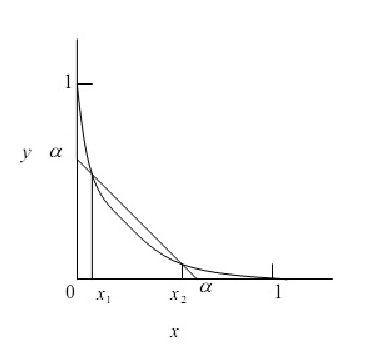
\includegraphics[width=0.5\hsize]{./img/log_relation.eps}
  \end{center}
  \caption{式(2.18)と式(2.19)の関係}
  \label{fig1}
\end{figure}

\newpage

\section{実験装置}
まず,図\ref{fig:config}及び表\ref{tab:spec}にレベル実験装置の構成及び仕様を示す.
\begin{table}[h]
  \begin{center}
    \caption{装置の仕様}
    \begin{tabular}{l|c|p{100mm}} \hline
      装置           & 数 & 仕様 \\ \hline
      タンク1        & 1  & 高さ$1000\,\mathrm{[mm]}$,内径$220\,\mathrm{[mm]}$ \\ \hline
      タンク2        & 1  & 高さ$1500\,\mathrm{[mm]}$,内径$320\,\mathrm{[mm]}$ \\ \hline
      電流比例制御弁 & 3  & 弁開度信号入力:$4〜20\,\mathrm{[mA]}$,全開-全閉時間:$17\,\mathrm{[s]}$以下,\newline 電源:$24\,\mathrm{[VDC]} \pm 10 \%$ \\ \hline
      流量計         & 3  & オープンコレクタ出力,$0.1\,\mathrm{[l/Pulse]}$ \\ \hline
      差圧変換器     & 2  & 容量:$200\,\mathrm{[gf/cm^2]}$ \\ \hline
      A/D変換ボード  & 1  & 入力:8CH,$0〜10\,\mathrm{[V]}$,分解能:$12\,\mathrm{[bit]}$ \\ \hline
      D/A変換ボード  & 1  & 出力:4CH,$4〜20\,\mathrm{[mA]}$,分解能:$12\,\mathrm{[bit]}$,変換速度:$10\,\mathrm{[\mu s/CH]}$ \\ \hline
      パルスカウンタ & 1  & 4CH,$24\,\mathrm{[bit]}$ up/down counter,外部入力:非絶縁TTL入力 \\ \hline
      コンピュータ   & 1  & NEC PC9801RX \\ \hline
    \end{tabular}
    \label{tab:spec}
  \end{center}
\end{table}

計算機からD/A変換器を介して入力される電流値によって制御バルブMV1の開度が変化し,
このバルブ開度に対応した流量の水がタンク1に入り
手動バルブを介してタンク2に流入する.
また,タンク2から制御バルブMV3を介して水が排出される.
これら入出流量に依存するタンクの水位は差圧変換器によって計測され,
D/A変換器を介して計算機に伝送される.\\

\begin{figure}[b]
  \begin{center}
    \includegraphics[width=0.8\hsize]{./img/system_config.eps}
  \end{center}
  \caption{実験装置の構成}
  \label{fig:config}
\end{figure}

 \section{実験方法}
以下の手順で実験準備を行った.
ただし,以下の手順1から5は実験指導担当者が行った.
\begin{enumerate}
  \item 配電盤のレベル系のスイッチを入れる.
  \item コンピュータの電源を入れる.
  \item 実験装置の電源スイッチを入れる.
  \item 給水用バルブ$V_1$を開く.
  \item 実験用プログラムを起動して以下の操作を行う.
        本実験ではUSER3のホームディレクトリexp3に格納されている下記の2種のプログラムを使用する.
    \begin{enumerate}
      \setlength{\leftskip}{5mm}
      \item \texttt{expapp}:差圧変換器特性の調査実験と流量の調整,タンク2の水抜きを行う.
      \item \texttt{step}:開ループ実験用プログラム.
    \end{enumerate}
  \item プログラム\texttt{expapp}を実行し以下の操作を行う.
    \begin{enumerate}
      \setlength{\leftskip}{5mm}
      \item 排水用電磁弁MV3への入力を$20 \, \mathrm{[mA]}$とし全開にする.
      \item 入水用電磁弁MV1への入力を$20 \, \mathrm{[mA]}$とし全開にする.
      \item 流量計の指示値が$30 \, \mathrm{[l/min]}$になるように手動でバルブ$V_1$を調整する.
    \end{enumerate}
    操作用コンピュータのディスプレイに表示される図中の記号の意味を表\ref{tab:display}に示す.
\end{enumerate}

\begin{table}[h]
  \begin{center}
    \caption{\texttt{expapp}における表示の意味}
    \begin{tabular}{c|l|l} \hline
      表記                      & 意味                              & 備考 \\ \hline
      MV1                       & タンク1注水用電磁バルブ指令電流値 & $4 \,\mathrm{[mA]}$から$20 \,\mathrm{[mA]}$ \\ \hline
      MV2                       & タンク2注水用電磁バルブ指令電流値 & $4 \,\mathrm{[mA]}$から$20 \,\mathrm{[mA]}$ \\ \hline
      MV3                       & タンク2排水用電磁バルブ指令電流値 & $4 \,\mathrm{[mA]}$から$20 \,\mathrm{[mA]}$ \\ \hline
      SAMPLING                  & サンプリング時間                  & $1 \,\mathrm{[s]}$から$3 \,\mathrm{[s]}$まで三段階で設定可能 \\ \hline
      APPLY                     & 設定値の変更を適用                & \\ \hline
      SV$\ast \,\mathrm{[mA]}$  & 電磁バルブ指令電流の設定値        & 実験前に表示 \\ \hline
      PV$\ast \,\mathrm{[mA]}$  & 電磁バルブ指令電流の現在地        & 実験中に表示 \\ \hline
      $\ast \,\mathrm{[l/min]}$ & 流量値                            & \\ \hline
      $\ast \,\mathrm{[V]}$     & 差圧変換器出力                    & \\ \hline
      IN                        & 入水経路                          & \\ \hline
      OUT                       & 排水経路                          & \\ \hline
    \end{tabular}
    \label{tab:display}
  \end{center}
\end{table}


\subsection{差圧変換器特性の調査実験}

以下の手順で差圧変換器特性の調査実験を行った.
\begin{enumerate}
  \item プログラム\texttt{expapp}を起動する.
  \item タンク2の定常水位が目的の初期水位となるよう入水用制御弁MV2を調整する.
  \item 目的の定常水位におけるタンク2の差圧変換器出力電圧を記録する.
  \item 手順(2)と(3)を水位がおよそ$60 \, \mathrm{[cm]}$となるまで繰り返す.
  \item 差圧変換器の出力電圧と水位の関係のグラフを描く.
\end{enumerate}

\subsection{ステップ応答実験}

以下の手順でステップ応答実験を行った.
\begin{enumerate}
  \item プログラム\texttt{step}を起動する.
  \item プログラムの指示に従い(1)制御弁の初期値,(2)変化量,(3)サンプリング周期を入力する.
  \item \texttt{[APPLY AND START]}をクリックして実験を開始する.
  \item タンク2の水位が定常値に収束した後に\texttt{[Recording Start]}をクリックする.
        10サンプルステップの後に手順(2)で与えた変化量の値だけさらに制御弁が開き,
        タンク2の差圧変換器出力の計測が開始される.
  \item 差圧変換器出力が定常値に収束した後に\texttt{[STOP]}をクリックし,データを保存する.
\end{enumerate}

 \section{結果}
 \subsection{差圧変換器特性の調査実験}
タンク2の水位と出力電圧を0[cm]から58[cm]まで5[cm]ごとに記録した.その結果を表\ref{tab1},図\ref{fig3}に示す.
\begin{table}[hb]
\centering
\caption{差圧変換器特性の実験結果}
\label{tab1}
 \begin{tabular}{|c|c|} \hline
  水位 & 出力電圧 \\ \hline \hline
  0	& -0.14 \\ \hline
  4.8	& 0.374 \\ \hline
  9.8	& 0.901 \\ \hline
  14.9	& 1.385 \\ \hline
  20	& 1.883 \\ \hline
  25	& 2.352 \\ \hline
  30.1	& 2.947 \\ \hline
  35	& 3.455 \\ \hline
  40.1	& 4.022 \\ \hline 
  45.4  & 4.564 \\ \hline 
  50.3	& 5.106 \\ \hline
  55.1	& 5.624 \\ \hline
  58	& 5.951 \\ \hline
 \end{tabular}
\end{table}
\newpage
\begin{figure}[hb]
 \begin{center}
  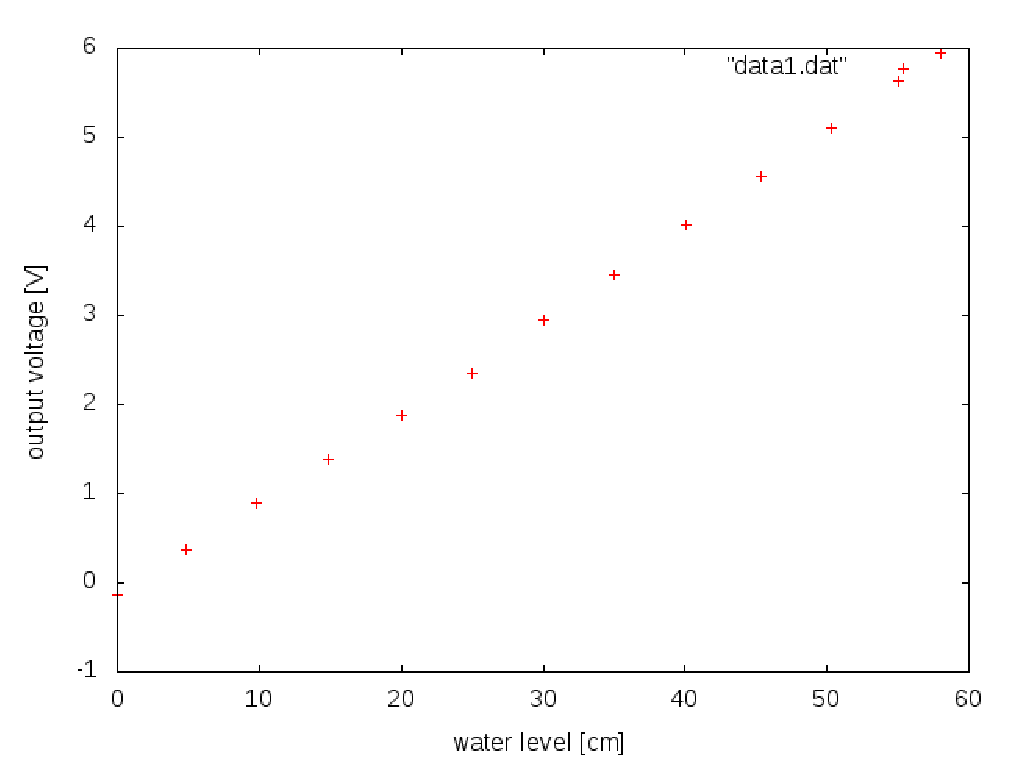
\includegraphics[scale = .7]{./picture/data1.eps}
 \end{center}
\end{figure}

\newpage

\subsection{ステップ応答実験}
制御弁の初期値を8$[mA]$,変化量を$1[mA]$,サンプリング周期を$5[sec]$として実験を行った. \\
 得られたデータより時間-流入量グラフと時間-出力電圧のグラフを作製した.それぞれ図\ref{fig4},\ref{fig5}に示す.
\begin{figure}[h]
 \begin{center}
  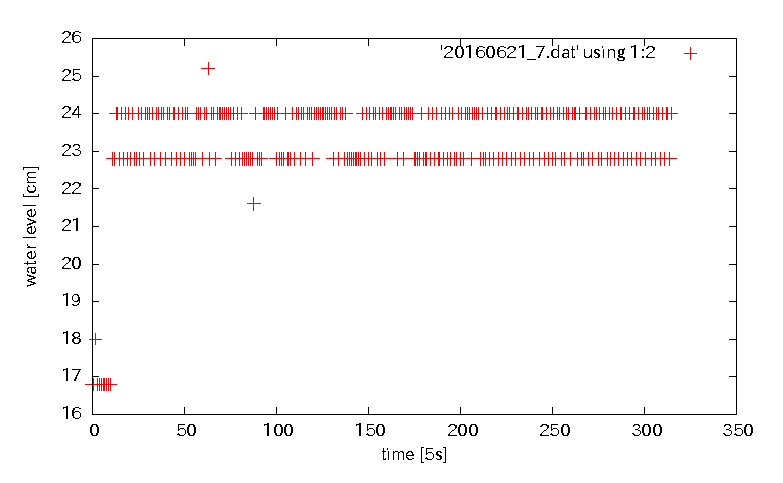
\includegraphics[scale = 1]{./picture/data2_1.eps}
 \end{center}
\caption{時間-流入量グラフ}
\label{fig4}
\end{figure}

\begin{figure}[h]
 \begin{center}
  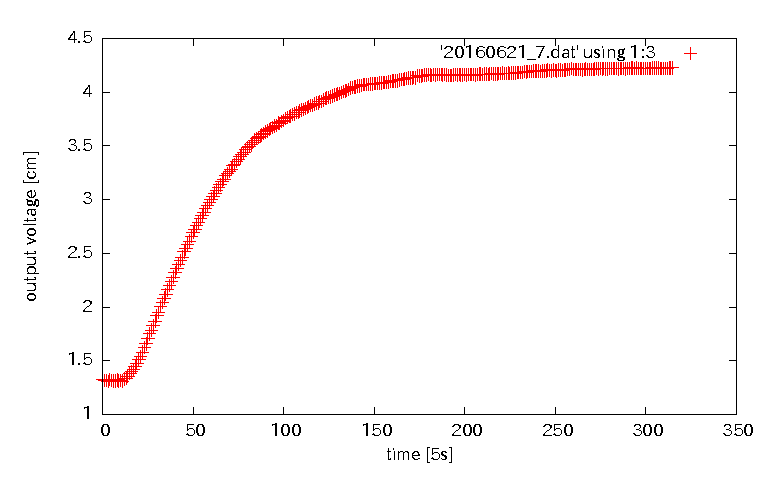
\includegraphics[scale = 1]{./picture/data2_2.eps}
 \end{center}
\caption{時間-出力電圧グラフ}
\label{fig5}
\end{figure}

\newpage

 \section{考察及び課題}
  \subsection{差圧変換器特性の調査実験について}
  得られたデータより,最小二乗法を用いて近似直線を求める.
図\ref{fig:data1}のグラフについて$y = a x + b$とおくと,
最小二乗法より$a$,$b$はそれぞれ以下のように表せる.
\begin{eqnarray}
  a &=& \frac{n \Sigma x_i y_i - \Sigma x_i \Sigma y_i}{n \Sigma {x_i}^2 - ( \Sigma x_i )^2} \\
  b &=& \frac{\Sigma {x_i}^2 \Sigma y_i - \Sigma x_i y_i \Sigma x_i}{n \Sigma {x_i}^2 - ( \Sigma x_i )^2}
\end{eqnarray}
これらの式より,$a \simeq 0.1046$,$b \simeq -0.1714$となり,
よって,差圧変換器出力-水位特性の関係式は,
\begin{equation}
  y = 0.1046x - 0.1714
\end{equation}
である.実験1のデータ点と共にグラフに表したものを図\ref{fig6}に示す.

\newpage

\begin{figure}[htb]
 \begin{center}
  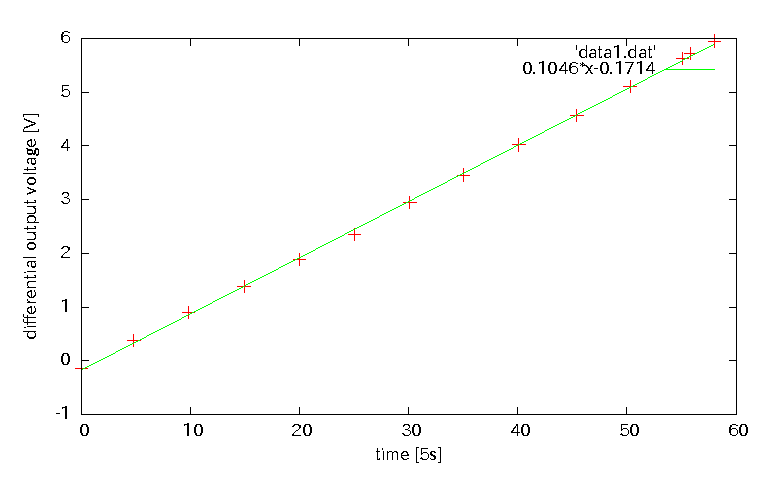
\includegraphics[scale = 1]{./picture/data1_2.eps}
 \end{center}
\caption{差圧変換器特性の調査実験の結果と近似曲線}
\label{fig6}
\end{figure}

\newpage

\thispagestyle{fancy}
\rhead{再1}
\cfoot{}

\subsection{差圧変換器特性について}
図\ref{fig5}の変曲点を見つけるためにそれぞれの点において次の点との差をとり,それが最も大きい点を変曲点とした.これより,変曲点を$T_c = 155$[sec]とした.これより,接線は
\begin{equation}
 y = ax + 1.321 - 31a
\end{equation}
と求まる.接線として相応しいaを設定し,$a = 0.03$とした.これと$y = 4.227,y = 1.321$との交点より,$t_a, t_b$を求めると,$t_a = 50, t_b = 534$となり,これより$T_A, T_C$は以下のようになった.
\begin{eqnarray}
 T_A & = & t_b - t_a = 484 \\
 T_C & = & t_b - t_c = 379
\end{eqnarray}
 式16より,$\alpha \simeq 0.783$となる.ここで,式19は解析的な解を求めるのが困難なため,表2よりデータをプロットし,$y = 0.783 - x$との交点における$x_1,x_2$をグラフより求める.結果をグラフに表した物を図\ref{fig7}に示す.

\begin{figure}[h]
 \begin{center}
  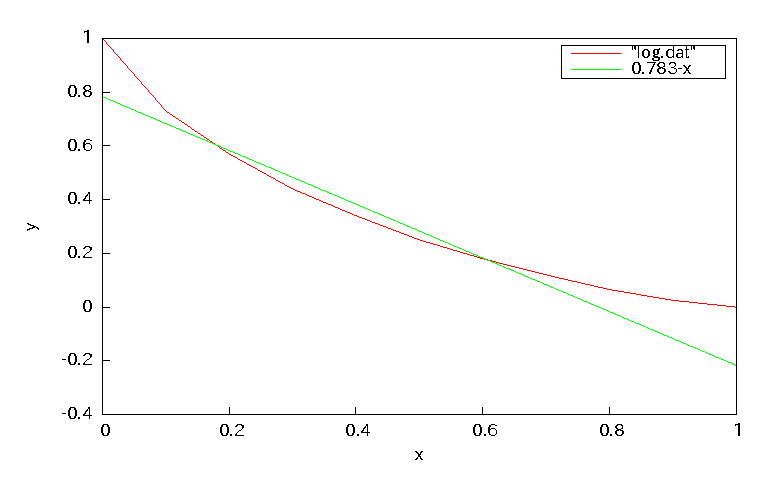
\includegraphics[scale = 1]{./picture/log.eps}
 \end{center}
\end{figure}

これより,$x_1 = 0.19,x_2 = 0.6$として,式18,19より$T_1,T_2$を求めると,$T_1 = 91.96$,$T_2 = 290.4$である.
 式3より,$t \to \infty$として,
\begin{equation}
 h(\infty) = rK = 4.227 - 1.321 = 2.906
\end{equation}


\newpage
\pagestyle{fancy}
\renewcommand{\headrulewidth}{0.0pt}
\rhead{再々1}
\cfoot{}
\setcounter{section}{4}
 \section{結果}
  \subsection{差圧変換器特性の調査実験}
  実験で得られたグラフを図\ref{fig8}に示す.
 \begin{figure}[h]
 \begin{center}
  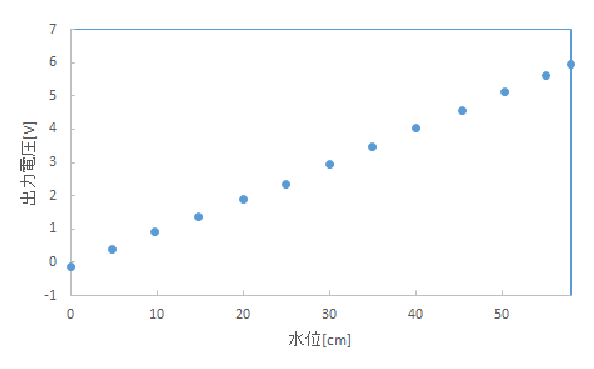
\includegraphics[scale=1]{./picture/e6_1.eps}
  \caption{差圧変換器の出力電圧と水位の関係}
  \label{fig8}
 \end{center}
 \end{figure}

\newpage
\pagestyle{fancy}
\renewcommand{\headrulewidth}{0.0pt}
\rhead{再々2}
\cfoot{}
  \subsection{ステップ応答実験}
  得られたグラフを図\ref{fig9},\ref{fig10}に示す.
\begin{figure}[h]
 \begin{center}
  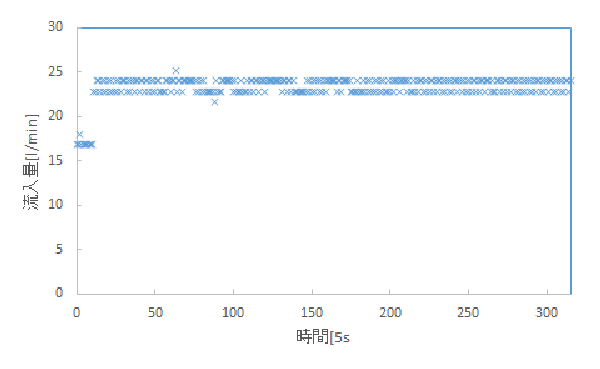
\includegraphics[scale=1]{./picture/e6_5.eps}
  \caption{時間-流入量グラフ}
  \label{fig9}
 \end{center}
\end{figure}

\begin{figure}[h]
 \begin{center}
  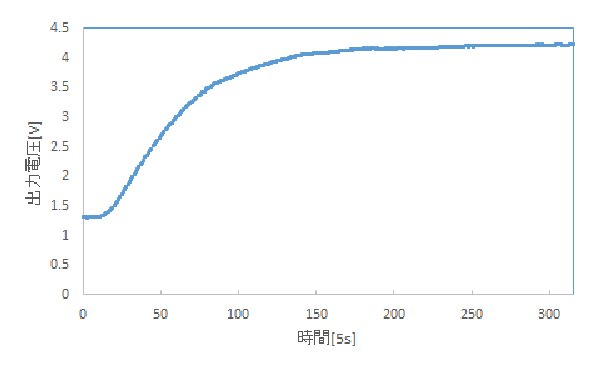
\includegraphics[scale=1]{./picture/e6_4.eps}
  \caption{時間-出力電圧グラフ}
  \label{fig10}
 \end{center}
\end{figure}

\newpage
\pagestyle{fancy}
\renewcommand{\headrulewidth}{0.0pt}
\rhead{再々3}
\cfoot{}

 \section{考察について}
  \subsection{差圧変換器特性の実験結果について}
  求めた近似直線をグラフにしたものを図\ref{fig11}に示す.
  \begin{figure}[h]
   \begin{center}
    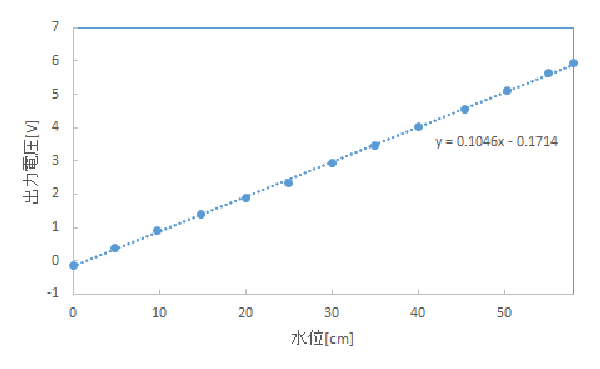
\includegraphics[scale=1]{./picture/e6_2.eps}
    \caption{差圧変換器特性の調査実験の結果と近似曲線}
    \label{fig11}
   \end{center}
  \end{figure}

\newpage
\pagestyle{fancy}
\renewcommand{\headrulewidth}{0.0pt}
\rhead{再々4}
\cfoot{}

  \subsection{差圧変換器特性について}
  $\alpha = 0.783$より,式19との関係をグラフにしたものを図\ref{fig12}に示す.
\begin{figure}[b]
 \begin{center}
  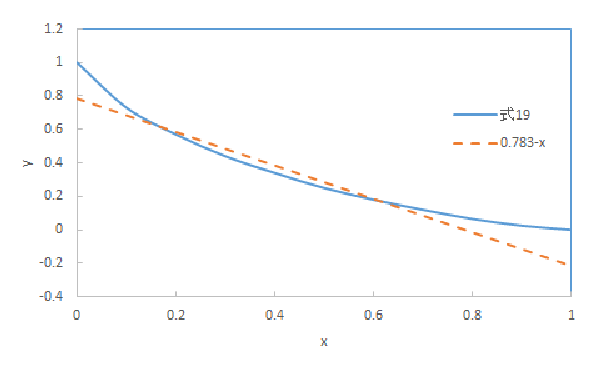
\includegraphics[scale=1]{./picture/e6_3.eps}
  \caption{式19と$y = 0.783-x$}
  \label{fig12}
 \end{center}
\end{figure}


式26より
\begin{equation}
 h(\infty) = rK = 4.227 - 1.321 = 2.906
\end{equation}
ここで,図\ref{fig9}より,$r = (23.5-16.8) \div 60 = 0.11$として,$K \simeq 26.18$.\\
よって,流入量から差圧変換器出力への伝達関数$G_1(s)$は
\begin{equation}
 G_1(s)= \frac{26.18}{(1+91.96s)(1+290.4s)}
\end{equation}
である.

\newpage
\pagestyle{fancy}
\renewcommand{\headrulewidth}{0.0pt}
\rhead{再々5}
\cfoot{}

  \subsection{流入量から水位への伝達関数}
  実験1および2の結果から,流入量を入力,
  タンク2の水位を出力とした伝達関数$G_2(s)$を求める.
  伝達関数は初期値を0と置くため,式22より
  \begin{equation}
   v(t) = 0.1046 h(t)
  \end{equation}
  である.これをラプラス変換すると
  \begin{equation}
   V(s) = 0.1046H(s)
  \end{equation}
  となる.これより,伝達関数$G_2(s)$は
\begin{equation}
 G_2(s)=\frac{H(s)}{U(s)}=\frac{H(s)}{V(s)} G_1(s) \simeq \frac{250.3}{(1+91.96s)(1+290.4s)}
\end{equation}
となる.

  \subsection{伝達関数の妥当性}
  求めた伝達関数について,$G_2(s)$に大きさ$r=0.11$のステップ入力を加えたときの時間応答は,初期値も考慮して,
\begin{eqnarray*}
 h(t) & = & 2.906(1+\frac{91.96}{290.4 - 91.96} e^{-\frac{t}{91.96}} - \frac{290.4}{290.4 - 91.96} e^{-\frac{t}{290.4}}) - 0.1714 \\
 & = & 29.06(1+0.783e^{-\frac{t}{91.96}} - 1.783 e^{-\frac{t}{290.4}}) + 14.2
\end{eqnarray*}
となった.\\
この式から時間-水位グラフを作成し,また差圧変換器-水位特性の近似直線を用いて実験で得られたデータから時間-水位グラフを作成した.図\ref{fig13}に示す.グラフより,定常値には大きな誤差は見られないが,立ち上がり時間において誤差が大きくなっている.また,立ち上がり時間は同定結果のほうが遅い.つまり,同定した伝達関数はゲインに関しては精度よく同定できているが,時定数については実際よりも小さいことがわかる. \\
時定数に誤差が生じた原因としては式19の解析解を求めることが困難なためにデータ点を用いたことや,$T_1,T_2$を求めるためにグラフから$x_1,x_2$を求める際に誤差が生じたためと考えられる.

\newpage
\pagestyle{fancy}
\renewcommand{\headrulewidth}{0.0pt}
\rhead{再々6}
\cfoot{}


\begin{figure}[H]
 \begin{center}
  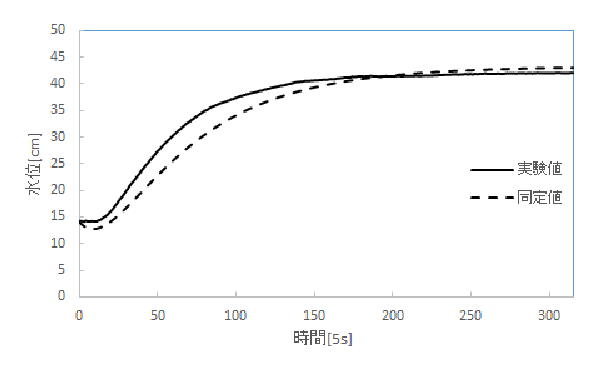
\includegraphics[scale=1]{./picture/e6_6.eps}
  \caption{実験値と同定値}
  \label{fig13} 
 \end{center}
\end{figure}



\section{まとめ}
レベル系の同定実験を行うことで,プロセス系への理解が深まった.


\newpage
\pagestyle{fancy}
\renewcommand{\thepage}{$付録$}
\renewcommand{\headrulewidth}{0.0pt}
\rhead{\thepage}
\lhead{}
\cfoot{}

\begin{longtable}[c]{|c|c|c|}
  \caption{実験結果}
  \label{tab6} \\
  \hline
   時間[5s] & 流入量[${\rm m^2/s}$]&	出力電圧[V]  \\ \hline \hline \endfirsthead 
\hline \endhead
\hline \endfoot
\hline \endlastfoot
0.000	&16.800&1.321  \\ \hline 	
1.000	&16.800&1.316  \\ \hline 	
2.000	&18.000&1.316  \\ \hline 	
3.000	&16.800&1.306  \\ \hline 	
4.000	&16.800&1.326  \\ \hline 	
5.000	&16.800&1.316  \\ \hline 	
6.000	&16.800&1.311  \\ \hline 	
7.000	&16.800&1.311  \\ \hline 	
8.000	&16.800&1.321  \\ \hline 	
9.000	&16.800&1.311  \\ \hline 	
10.000	&16.800&1.316  \\ \hline 	
11.000	&22.800&1.311  \\ \hline 	
12.000	&22.800&1.331  \\ \hline 	
13.000	&24.000&1.336  \\ \hline 	
14.000	&24.000&1.355  \\ \hline 	
15.000	&22.800&1.380  \\ \hline 	
16.000	&24.000&1.399  \\ \hline 	
17.000	&22.800&1.419  \\ \hline 	
18.000	&24.000&1.443  \\ \hline 	
19.000	&22.800&1.477  \\ \hline 	
20.000	&24.000&1.507  \\ \hline 	
21.000	&22.800&1.541  \\ \hline 	
22.000	&24.000&1.580  \\ \hline 	
23.000	&22.800&1.624  \\ \hline 	
24.000	&22.800&1.658  \\ \hline 	
25.000	&24.000&1.707  \\ \hline 	
26.000	&22.800&1.751  \\ \hline 	
27.000	&24.000&1.785  \\ \hline 	
28.000	&22.800&1.824  \\ \hline 	
29.000	&24.000&1.868  \\ \hline 	
30.000	&24.000&1.917  \\ \hline 	
31.000	&24.000&1.951  \\ \hline 	
32.000	&22.800&2.005  \\ \hline 	
33.000	&24.000&2.044  \\ \hline 	
34.000	&22.800&2.083  \\ \hline 	
35.000	&24.000&2.117  \\ \hline 	
36.000	&24.000&2.161  \\ \hline 	
37.000	&22.800&2.200  \\ \hline 	
38.000	&24.000&2.234  \\ \hline 	
39.000	&24.000&2.278  \\ \hline 	
40.000	&22.800&2.322  \\ \hline 	
41.000	&24.000&2.357  \\ \hline 	
42.000	&24.000&2.400  \\ \hline 	
43.000	&22.800&2.435  \\ \hline 	
44.000	&24.000&2.464  \\ \hline 	
45.000	&24.000&2.513  \\ \hline 	
46.000	&22.800&2.542  \\ \hline 	
47.000	&24.000&2.586  \\ \hline 	
48.000	&22.800&2.615  \\ \hline 	
49.000	&24.000&2.659  \\ \hline 	
50.000	&22.800&2.694  \\ \hline 	
51.000	&24.000&2.718  \\ \hline 	
52.000	&24.000&2.757  \\ \hline 	
53.000	&22.800&2.791  \\ \hline 	
54.000	&22.800&2.825  \\ \hline 	
55.000	&22.800&2.855  \\ \hline 	
56.000	&22.800&2.884  \\ \hline 	
57.000	&24.000&2.913  \\ \hline 	
58.000	&24.000&2.943  \\ \hline 	
59.000	&24.000&2.972  \\ \hline 	
60.000	&22.800&3.006  \\ \hline 	
61.000	&24.000&3.031  \\ \hline 	
62.000	&24.000&3.060  \\ \hline 	
63.000	&25.200&3.089  \\ \hline 	
64.000	&22.800&3.114  \\ \hline 	
65.000	&24.000&3.138  \\ \hline 	
66.000	&24.000&3.172  \\ \hline 	
67.000	&22.800&3.192  \\ \hline 	
68.000	&24.000&3.226  \\ \hline 	
69.000	&24.000&3.245  \\ \hline 	
70.000	&24.000&3.265  \\ \hline 	
71.000	&24.000&3.284  \\ \hline 	
72.000	&24.000&3.314  \\ \hline 	
73.000	&24.000&3.328  \\ \hline 	
74.000	&24.000&3.358  \\ \hline 	
75.000	&24.000&3.377  \\ \hline 	
76.000	&22.800&3.397  \\ \hline 	
77.000	&24.000&3.421  \\ \hline 	
78.000	&22.800&3.441  \\ \hline 	
79.000	&24.000&3.465  \\ \hline 	
80.000	&22.800&3.485  \\ \hline 	
81.000	&24.000&3.495  \\ \hline 	
82.000	&22.800&3.509  \\ \hline 	
83.000	&22.800&3.534  \\ \hline 	
84.000	&22.800&3.553  \\ \hline 	
85.000	&22.800&3.568  \\ \hline 	
86.000	&22.800&3.578  \\ \hline 	
87.000	&22.800&3.592  \\ \hline 	
88.000	&21.600&3.602  \\ \hline 	
89.000	&24.000&3.617  \\ \hline 	
90.000	&22.800&3.631  \\ \hline 	
91.000	&22.800&3.641  \\ \hline 	
92.000	&22.800&3.651  \\ \hline 	
93.000	&24.000&3.661  \\ \hline 	
94.000	&24.000&3.670  \\ \hline 	
95.000	&24.000&3.685  \\ \hline 	
96.000	&24.000&3.690  \\ \hline 	
97.000	&24.000&3.714  \\ \hline 	
98.000	&24.000&3.709  \\ \hline 	
99.000	&24.000&3.729  \\ \hline 	
100.000	&22.800&3.739  \\ \hline 	
101.000	&24.000&3.753  \\ \hline 	
102.000	&22.800&3.763  \\ \hline 	
103.000	&22.800&3.773  \\ \hline 	
104.000	&22.800&3.778  \\ \hline 	
105.000	&24.000&3.792  \\ \hline 	
106.000	&22.800&3.797  \\ \hline 	
107.000	&22.800&3.812  \\ \hline 	
108.000	&22.800&3.812  \\ \hline 	
109.000	&24.000&3.827  \\ \hline 	
110.000	&22.800&3.836  \\ \hline 	
111.000	&24.000&3.841  \\ \hline 	
112.000	&24.000&3.846  \\ \hline 	
113.000	&22.800&3.856  \\ \hline 	
114.000	&24.000&3.866  \\ \hline 	
115.000	&24.000&3.875  \\ \hline 	
116.000	&22.800&3.875  \\ \hline 	
117.000	&24.000&3.890  \\ \hline 	
118.000	&24.000&3.900  \\ \hline 	
119.000	&24.000&3.900  \\ \hline 	
120.000	&22.800&3.915  \\ \hline 	
121.000	&24.000&3.915  \\ \hline 	
122.000	&24.000&3.929  \\ \hline 	
123.000	&24.000&3.939  \\ \hline 	
124.000	&24.000&3.944  \\ \hline 	
125.000	&24.000&3.949  \\ \hline 	
126.000	&24.000&3.958  \\ \hline 	
127.000	&24.000&3.963  \\ \hline 	
128.000	&24.000&3.973  \\ \hline 	
129.000	&24.000&3.978  \\ \hline 	
130.000	&24.000&3.983  \\ \hline 	
131.000	&22.800&3.988  \\ \hline 	
132.000	&24.000&3.998  \\ \hline 	
133.000	&24.000&4.007  \\ \hline 	
134.000	&22.800&4.012  \\ \hline 	
135.000	&24.000&4.017  \\ \hline 	
136.000	&24.000&4.027  \\ \hline 	
137.000	&22.800&4.037  \\ \hline 	
138.000	&24.000&4.046  \\ \hline 	
139.000	&22.800&4.051  \\ \hline 	
140.000	&22.800&4.051  \\ \hline 	
141.000	&22.800&4.056  \\ \hline 	
142.000	&22.800&4.056  \\ \hline 	
143.000	&22.800&4.061  \\ \hline 	
144.000	&22.800&4.071  \\ \hline 	
145.000	&22.800&4.071  \\ \hline 	
146.000	&22.800&4.071  \\ \hline 	
147.000	&24.000&4.071  \\ \hline 	
148.000	&22.800&4.076  \\ \hline 	
149.000	&24.000&4.076  \\ \hline 	
150.000	&22.800&4.081  \\ \hline 	
151.000	&24.000&4.081  \\ \hline 	
152.000	&22.800&4.081  \\ \hline 	
153.000	&24.000&4.085  \\ \hline 	
154.000	&24.000&4.085  \\ \hline 	
155.000	&22.800&4.090  \\ \hline 	
156.000	&24.000&4.090  \\ \hline 	
157.000	&22.800&4.090  \\ \hline 	
158.000	&24.000&4.095  \\ \hline 	
159.000	&22.800&4.100  \\ \hline 	
160.000	&24.000&4.105  \\ \hline 	
161.000	&24.000&4.105  \\ \hline 	
162.000	&24.000&4.105  \\ \hline 	
163.000	&24.000&4.105  \\ \hline 	
164.000	&24.000&4.115  \\ \hline 	
165.000	&24.000&4.120  \\ \hline 	
166.000	&22.800&4.120  \\ \hline 	
167.000	&24.000&4.125  \\ \hline 	
168.000	&24.000&4.129  \\ \hline 	
169.000	&22.800&4.134  \\ \hline 	
170.000	&24.000&4.134  \\ \hline 	
171.000	&24.000&4.134  \\ \hline 	
172.000	&24.000&4.139  \\ \hline 	
173.000	&24.000&4.134  \\ \hline 	
174.000	&24.000&4.154  \\ \hline 	
175.000	&22.800&4.149  \\ \hline 	
176.000	&22.800&4.149  \\ \hline 	
177.000	&22.800&4.154  \\ \hline 	
178.000	&22.800&4.159  \\ \hline 	
179.000	&24.000&4.159  \\ \hline 	
180.000	&22.800&4.164  \\ \hline 	
181.000	&22.800&4.159  \\ \hline 	
182.000	&22.800&4.154  \\ \hline 	
183.000	&24.000&4.164  \\ \hline 	
184.000	&22.800&4.159  \\ \hline 	
185.000	&24.000&4.164  \\ \hline 	
186.000	&22.800&4.164  \\ \hline 	
187.000	&24.000&4.164  \\ \hline 	
188.000	&22.800&4.159  \\ \hline 	
189.000	&22.800&4.164  \\ \hline 	
190.000	&24.000&4.159  \\ \hline 	
191.000	&22.800&4.154  \\ \hline 	
192.000	&24.000&4.154  \\ \hline 	
193.000	&22.800&4.154  \\ \hline 	
194.000	&24.000&4.159  \\ \hline 	
195.000	&22.800&4.164  \\ \hline 	
196.000	&24.000&4.159  \\ \hline 	
197.000	&22.800&4.164  \\ \hline 	
198.000	&22.800&4.159  \\ \hline 	
199.000	&24.000&4.159  \\ \hline 	
200.000	&22.800&4.164  \\ \hline 	
201.000	&24.000&4.159  \\ \hline 	
202.000	&22.800&4.164  \\ \hline 	
203.000	&24.000&4.164  \\ \hline 	
204.000	&24.000&4.164  \\ \hline 	
205.000	&24.000&4.164  \\ \hline 	
206.000	&22.800&4.159  \\ \hline 	
207.000	&24.000&4.164  \\ \hline 	
208.000	&24.000&4.168  \\ \hline 	
209.000	&24.000&4.168  \\ \hline 	
210.000	&24.000&4.164  \\ \hline 	
211.000	&22.800&4.168  \\ \hline 	
212.000	&24.000&4.168  \\ \hline 	
213.000	&22.800&4.164  \\ \hline 	
214.000	&22.800&4.168  \\ \hline 	
215.000	&24.000&4.173  \\ \hline 	
216.000	&22.800&4.168  \\ \hline 	
217.000	&24.000&4.168  \\ \hline 	
218.000	&22.800&4.168  \\ \hline 	
219.000	&24.000&4.173  \\ \hline 	
220.000	&24.000&4.173  \\ \hline 	
221.000	&22.800&4.178  \\ \hline 	
222.000	&24.000&4.173  \\ \hline 	
223.000	&22.800&4.173  \\ \hline 	
224.000	&24.000&4.178  \\ \hline 	
225.000	&22.800&4.173  \\ \hline 	
226.000	&24.000&4.178  \\ \hline 	
227.000	&24.000&4.178  \\ \hline 	
228.000	&22.800&4.178  \\ \hline 	
229.000	&24.000&4.183  \\ \hline 	
230.000	&22.800&4.183  \\ \hline 	
231.000	&24.000&4.183  \\ \hline 	
232.000	&24.000&4.183  \\ \hline 	
233.000	&22.800&4.193  \\ \hline 	
234.000	&24.000&4.188  \\ \hline 	
235.000	&22.800&4.193  \\ \hline 	
236.000	&24.000&4.193  \\ \hline 	
237.000	&24.000&4.193  \\ \hline 	
238.000	&22.800&4.198  \\ \hline 	
239.000	&24.000&4.198  \\ \hline 	
240.000	&22.800&4.198  \\ \hline 	
241.000	&24.000&4.198  \\ \hline 	
242.000	&24.000&4.193  \\ \hline 	
243.000	&22.800&4.198  \\ \hline 	
244.000	&24.000&4.198  \\ \hline 	
245.000	&24.000&4.198  \\ \hline 	
246.000	&22.800&4.208  \\ \hline 	
247.000	&24.000&4.203  \\ \hline 	
248.000	&22.800&4.198  \\ \hline 	
249.000	&24.000&4.208  \\ \hline 	
250.000	&22.800&4.203  \\ \hline 	
251.000	&24.000&4.198  \\ \hline 	
252.000	&22.800&4.208  \\ \hline 	
253.000	&24.000&4.208  \\ \hline 	
254.000	&24.000&4.203  \\ \hline 	
255.000	&22.800&4.208  \\ \hline 	
256.000	&24.000&4.208  \\ \hline 	
257.000	&22.800&4.212  \\ \hline 	
258.000	&24.000&4.212  \\ \hline 	
259.000	&24.000&4.222  \\ \hline 	
260.000	&22.800&4.212  \\ \hline 	
261.000	&24.000&4.212  \\ \hline 	
262.000	&24.000&4.212  \\ \hline 	
263.000	&24.000&4.212  \\ \hline 	
264.000	&22.800&4.212  \\ \hline 	
265.000	&24.000&4.208  \\ \hline 	
266.000	&22.800&4.212  \\ \hline 	
267.000	&22.800&4.217  \\ \hline 	
268.000	&24.000&4.212  \\ \hline 	
269.000	&24.000&4.212  \\ \hline 	
270.000	&22.800&4.212  \\ \hline 	
271.000	&24.000&4.212  \\ \hline 	
272.000	&22.800&4.217  \\ \hline 	
273.000	&24.000&4.222  \\ \hline 	
274.000	&24.000&4.217  \\ \hline 	
275.000	&22.800&4.222  \\ \hline 	
276.000	&24.000&4.217  \\ \hline 	
277.000	&22.800&4.222  \\ \hline 	
278.000	&24.000&4.217  \\ \hline 	
279.000	&24.000&4.217  \\ \hline 	
280.000	&22.800&4.222  \\ \hline 	
281.000	&24.000&4.222  \\ \hline 	
282.000	&22.800&4.222  \\ \hline 	
283.000	&24.000&4.222  \\ \hline 	
284.000	&22.800&4.222  \\ \hline 	
285.000	&24.000&4.217  \\ \hline 	
286.000	&22.800&4.222  \\ \hline 	
287.000	&24.000&4.222  \\ \hline 	
288.000	&24.000&4.222  \\ \hline 	
289.000	&22.800&4.217  \\ \hline 	
290.000	&24.000&4.222  \\ \hline 	
291.000	&22.800&4.222  \\ \hline 	
292.000	&24.000&4.227  \\ \hline 	
293.000	&22.800&4.227  \\ \hline 	
294.000	&24.000&4.222  \\ \hline 	
295.000	&24.000&4.227  \\ \hline 	
296.000	&22.800&4.222  \\ \hline 	
297.000	&24.000&4.222  \\ \hline 	
298.000	&22.800&4.222  \\ \hline 	
299.000	&24.000&4.222  \\ \hline 	
300.000	&24.000&4.222  \\ \hline 	
301.000	&22.800&4.222  \\ \hline 	
302.000	&24.000&4.222  \\ \hline 	
303.000	&24.000&4.222  \\ \hline 	
304.000	&22.800&4.227  \\ \hline 	
305.000	&24.000&4.227  \\ \hline 	
306.000	&22.800&4.227  \\ \hline 	
307.000	&24.000&4.227  \\ \hline 	
308.000	&24.000&4.222  \\ \hline 	
309.000	&22.800&4.222  \\ \hline 	
310.000	&24.000&4.222  \\ \hline 	
311.000	&22.800&4.222  \\ \hline 	
312.000	&24.000&4.222  \\ \hline 	
313.000	&24.000&4.227  \\ \hline 	
314.000	&22.800&4.227  \\ \hline 	
315.000	&24.000&4.227  \\ \hline
\end{longtable} 	


\end{document}





